\begin{abstract}
 The abstract goes here... (BITCOIN influence -> Blockchain). Captivate readers attention.
\end{abstract}




%*****************************************
\chapter{Introduction}
%*****************************************

Blockchain (BC) has been considered as one of the most promising disruptive technologies during the last years. Many market-leading companies, experts and global innovators have referred it as the "Next Generation of the Internet" \cite{JenClarck2017}, succeeding the World Wide Web era. Evaluating its potential benefits, different banks and major enterprises, such as UBS, Microsoft or IBM, have already accomplished important investments in such innovative technologies.

The revolution started in 2008, with a whitepaper publication by Satoshi Nakamoto \cite{nakamoto2008bitcoin}, who introduces a new digital payment protocol called Bitcoin. Satoshi Nakamoto is just a name used by an unknown person or group of people to first reference the implementation. Nowadays, Bitcoin's creator still remains a mystery.

In 2009, a deployed software version based on the paper was launched. Bitcoin uses an alternative virtual currency, to make trusted transactions between different peers. This system relies on a kind of distributed database allocated on the Internet, the blockchain. Blockchain uses a peer-to-peer architecture model combined with secure algorithms, such as public key cryptography, which intentionally removes the presence of middle-parties or intermediaries. Thus, in the case of Bitcoin, it eliminates the agent responsible for transactions: central banks.

At the beginning, the blockchain architecture was restricted to only one application: online payments. However, after observing its advantages and possible use cases, an improvement of Bitcoin emerged: Ethereum \footnote{\url{https://www.ethereum.org/}}. By contrast, Ethereum extends the power of decentralized transactions with a Turing-complete contract system. A Turing-complete system can perform any computation, with just writing a few lines of code, in order to create Ethereum scripts: smart contracts. A smart contract can be generated with non-restrictive and user-friendly programming languages, allowing developers to easily learn and benefit from them. Therefore, it brings to the user the opportunity to develop their own applications. Smart contracts are used to implement decentralized apps, which unlike normal web apps, they may not be allocated in a central server. In other words, they use blockchain technology to retrieve and store data instead of a database.


\section{Motivation}

Nowadays, blockchain is becoming a trending topic in the business world. Thousands of articles, research papers and books, such as: How the technology behind bitcoin is changing money, business and the world \cite{tapscott2016blockchain} or Blockchain: Blue print for a new economy \cite{swan2015blockchain}, are catching the public eye. Nevertheless, as it is an emerging technology, a necessity to look towards new horizons exists. Through the use of the above mentioned Ethereum smart contracts new possibilities to approach existing problems are opened up. Hence, blockchain technology can be used in many applications beyond currency.

Many scenarios are currently investigated from a blockchain perspective, e.g: candidate's voting or asset tracking \cite{abeyratne2016blockchain}. In the former, voters send signed and encrypted ballots to the blockchain contract, who immediately verifies them. Simultaneously, it also preserves confidentiality, since the ballot can only be emitted from its owner. In the latter, each physical asset could be encoded in the blockchain enabling a fast and transparent tracking. For example, Everledger \footnote{\url{https://www.everledger.ioafa}}, a startup company from London, tracks diamonds storing each diamond's digital identity on the BC. Thus, diamond theft could be effectively prevented.

After investigating the implementation of blockchain in real scenarios, one top-level application is clear: it can be used as a software connector. Blockchain contributes to face security, storage's problem, communication and coordination between users. In this paper, we will focus on enterprises or organizations, suffering from such problem, referenced from now on as supply chain challenges.

\section{Problem Statement and Contribution}

Supply chain management is the process of linking organizations through information flows, in order to achieve a competitive strength or advantage, which will maximise customer value. Supply chain activities go from the design or development of a product, up to its return on investment (ROI). Thus, a good coordination during these activities is extremely needed.

Nowadays in the Big Data era, enterprises must handle a huge amount of information. This leads companies to suffer from considerable issues, such as scalability, data's security or communication. One could think that currently most of these companies rely on third parties, which help them on the mentioned problems. But what if this process could be efficiently accelerated in a secure and decentralized manner? Here, is where Blockchain can play a crucial role.

During the paper, the focus will be on IT companies facing this dilemma. The scenario will include in one side different customers, and in the other organizations acting as providers. For example, eBay, one of the biggest multinational e-commerce corporations, acts as an intermediate for the product's purchase-sale. Thus, eBay is responsible for managing all this data. However, can a user/company always safely trust third-parties? Why not using BC as the main responsible for handling such complex tasks? This will result in a direct customer-provider relation, avoiding the presence of any intermediaries.

For this scenario, a current application example that consists of the embedding of virtual networks (network virtualization) between different Infrastructure Providers (InPs), will be further investigated \cite{dietrich2015multi}. This process can also be called network slicing. In this example, Service Providers (SPs) want to embed virtual nodes among different InPs. Nevertheless, Infrastructure Providers are not willing to publicly disclose its internal network topology, along with its resources availability and costs. In such cases, brokers, usually known as VN Providers (VNP) try to perform the embedding under the mentioned limited information disclosure (LID) problem. As a result, it can be clearly observed that blockchain can solve this interaction, providing: secure sensitive data storage, customer-provider negotiation without third-parties (without VNP) and finally maintaining a coordinated process. The negotiation between the involved parties will be based on a time-limited auction system, where each virtual network request will be stored as a contract on the blockchain network.

Therefore, a good question for the theses could be: How blockchain takes advantage of distributed workflows providing an agile and secure environment? Exemplifying workflows, with the network slicing example. At the end, a decentralized application approaching the mentioned problem will be deployed. In addition, the app will include a user-friendly front-end in order to guide users through the process. 


\section{Outline}

How is the rest of this thesis structured?


%*****************************************
\chapter{Background}
\label{ch:background}
%*****************************************

In this section, an overview of the blockchain technology evolution along will be provided. It starts with the 1st blockchain generation related to cryptocurrencies, with Bitcoin as a leading representative. Then, the second or smart contracts generation will be investigated, where Ethereum extends the idea of money transfers, to any other application that can be writable as a piece of code.

Afterwards, our scenario will be introduced, which focuses on network virtualization. In this environment, resource negotiation between customer and providers is crucial, which will be accomplished through a limited time auction. Thus, the pros and cons of different types of auctions will also be discussed.

\section{Blockchain: A decentralized and distributed trustless ledger}

What is a blockchain? A blockchain is a decentralized distributed ledger, which stores the entire history of transactions on the network. In other words, it is a simple database distributed among a network of computers, where each computer has an identical copy of this database. This contrasts with traditional (e.g. SQL) databases that are controlled by a single entity. Thus, in a blockchain, there is no central server or agent in the middle of the communication (Figure \ref{fig:CentralizedvsDecentralized}).

And why is a blockchain better than a traditional database? The truth of it is that there is no better technology than the others, it just depends on user's requirements. However, blockchain provide multiple advantages such as: \newline
\textbf{(i) Disintermediation:} Running without a central administrator. This is possible because it uses its own consensus mechanisms, such as the Proof-of-Work (later explained). \newline
\textbf{(ii) Privacy:} Data is encrypted and stored on the blockchain, and it also requires user authentication. \newline
\textbf{(iii) Robustness:} Different databases do not need to be synchronized across different boundaries. All the information is stored in a single blockchain. \newline 
\textbf{(iv) Transparency:} All the transactions are logged on the system. \newline 
A good example where all these requirements are needed is in the healthcare environment. There, patient records are stored in multiple databases, which always leads to a costly exchange of information between them. In this scenario, the blockchain could improve the process, preserving at the same time security and patients confidentiality.


\begin{figure}
  \centering
  	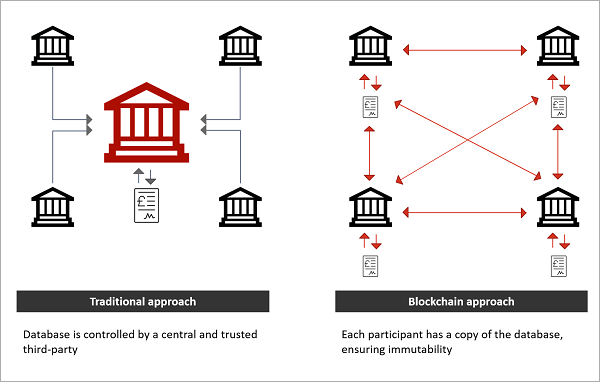
\includegraphics[scale=0.8]{gfx/centralization_vs_decentralization.png}
  \caption{Traditional database vs blockchain approach}
  \label{fig:CentralizedvsDecentralized}
\end{figure}

Returning to the Bitcoin concept, at the beginning, the terms Bitcoin and blockchain were sometimes interchanged, as these words were used to refer: (i) the technology, (ii) the protocol for making transactions and (iii) the cryptocurrency (money). Therefore, before starting there is one statement that needs to be clear: Bitcoin is a cryptocurrency that uses the blockchain technology. Hence, Bitcoin is just one of the multiple applications that use blockchain. 

However, when a new technology appears, the first user's goal is normally to exploit its economic potential. Therefore, money transaction through cryptocurrencies was its first application. In the next subsection, we will understand what cryptocurrencies really are, followed by an explanation of the architectural design of the Bitcoin idea along with its implications.

\subsection{Blockchain 1.0: Cryptocurrencies}

At of the end of January 2018, Coinmarketcap, a cryptocurrency market tracker, lists more than 1,400 cryptocurrencies with an aggregate value approaching USD 700bn.  But what are cryptocurrencies? Cryptocurrencies are a variety of digital currencies pretending to work as a medium of exchange, such as Euro or USD does. As the name suggests, apart from being a virtual currency, they use cryptography to secure and verify its transactions. The main difference with traditional currencies is that they do not have any physical equivalent in the real world. Nevertheless, they can be used to pay goods and service, with the advantage of not having any geographical or political borders. For example, GMO Internet, a Japanese company, will start paying parts of employees salaries in cryptocurrencies (Bitcoin).

In this paper, we will set aside whether they can become true currencies or not, and also its political, social or economic impact. The only focus will be the technology behind it, as blockchain can be extended to much more than digital currencies. Thus, we will start from the genesis of the technology, with Bitcoin as its revolutionary innovator.


\subsubsection{Bitcoin}

Bitcoin took the world by surprise in 2009, after Satoshi Nakotomo's white paper publication \cite{nakamoto2008bitcoin} and later its software release. Bitcoin is a cryptocurrency used for making secure transactions across a peer-to-peer (P2P) network. In addition, Bitcoin uses its own protocol that operates in an overlay network, the blockchain. An overlay network is a computer network build in the top of another network, in this case above Internet application's layer.

Furthermore, in Bitcoin, each user possesses a digital Wallet, which is a software program used for performing the transactions. Each of these users is identified by a single public address, composed of 26-35 alphanumeric characters, which is the hash of the user's public key. For example, if user A wants to send Bitcoins to user B, it needs B public address, e.g: 1BvBMSEYstWetqTFn5Au4m4GFg7xJaNVN2. Then, user A creates a message (transaction), attaching receiver's public key with the transferred amount of Bitcoins. This message is signed by sender's private key and sent to the blockchain. Transactions examples can be found in \footnote{\url{https://blockexplorer.com/}}.

From another point of view, the Bitcoin ledger can be interpreted as a state transition system, where there is an initial state, which after a transition function (money transfer), results in a new state. Imagine the last example where A wants to send X to B. The first state is A and B current balance and the transition function will take X from A and insert it to B's account, generating a new state. But what happens if A sends exactly the same payment to two different addresses (B and C) at the same time? This scenario is the so-called double spending attack and consequently, a transaction always needs to be verified by miners in the blockchain before being confirmed.

And how all these miners cooperate efficiently? The answer to this question is one of the most remarkable Satoshi innovation key factors, which consists of the communication between nodes through a simple decentralized \textbf{ consensus protocol}. This consensus protocol consists of multiple algorithms (e.g. Proof of Work), used by specific peers in the Bitcoin network. These peers, also called miners, are responsible for monitoring and verifying all the transactions between users.

\paragraph{Mining}

Bitcoin needs to combine the state transition system with a consensus protocol, to synchronize the order of all transactions among the users.
New transactions are stored in the last block of the blockchain, and a new block is mined every ten minutes. Over time, this creates an ever-growing chain of blocks, which are constantly updated. Thus the name: blockchain. Additionally, a complete history of the transactions is kept, so everyone can verify the last money movements. For instance, a blockchain can be compared to an endless domino game, where all the pieces are placed in vertical one after the other. Each of these pieces references a block, and if one block is not placed correctly (block's error), all the subsequent ones will be affected. Therefore, miner's task is not simple and requires computational power.

\begin{figure}
  \centering
  	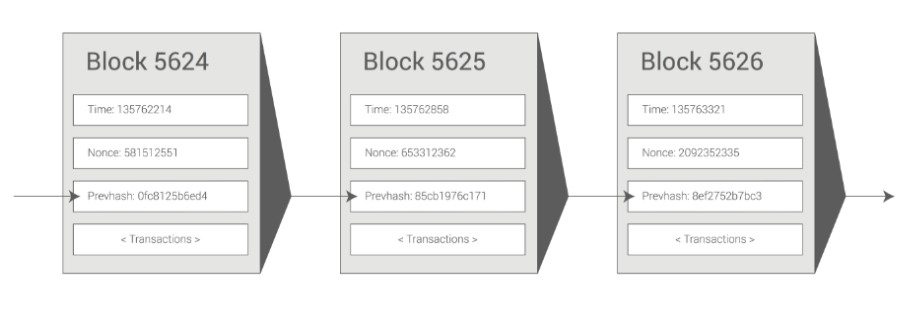
\includegraphics[scale=0.5]{gfx/mining.png}
  \caption{Bitcoin Mining}
  \label{fig:Bitcoin mining}
\end{figure}

Figure \ref{fig:Bitcoin mining} shows a chain of blocks, where each block contains (i) a timestamp, (ii) a nonce, a (iii) hash reference to the previous block and (iv) a list of all the transactions that have been created since the previous block. Thus, for a block being valid needs to satisfy the following requirements: \newline (i) Previous block referenced exists. (ii) Block's timestamp is greater than previous block one. (iii) Proof-of-work in this block is valid. (iv) If any transaction from the transaction lists returns an error, exit. (v) If all previous steps confirmed, store state at the end of the block and return true.

In the third step of the block validation process, appears the term Proof-of-work. Bitcoin uses the Hashcash proof of work algorithm to prove that a block miner spent some computational time creating a block. In particular, the algorithm works with cryptographic hashes, such as SHA1 or SHA256. Proof-of-work is also used in other contexts, such as limiting email spam or denial-of-service attacks (DoS). This technique can lead to a low probability so that the only way to create a valid block is simply trial and error until a valid Proof-of-Work is generated.

Nevertheless, as miners must perform a high computational work, they receive a reward for the mining process. Additionally, if any transaction has a positive balance at the end, it is also destinated to the miner.


\subsection{Blockchain 2.0: Smart contracts}

The Blockchain 1.0 had numerous limitations since essentially it only approaches the decentralization of money and payments. However, the architecture implemented by Bitcoin is extensible beyond financial uses cases.

\subsubsection{Ethereum}

In 2013 Vitalik Buterin, a Russian-Canadian programmer released the Ethereum white paper \cite{buterin2014next}, where he describes an alternative platform running in a blockchain that allows building any kind of decentralized application. In 2014 Ethereum started as a crowdfunding project, which collects small amounts of money from a large number of users.  Ethereum is currently a running project and the second most valuable cryptocurrency.

Furthermore, it is built on a Turing-complete contract system. As previously explained, a Turing-complete system allows the developer to perform any computation, which runs on the so-called \textbf{smart contracts}. These smarts contracts are executed by the Ethereum nodes, each using its Ethereum Virtual Machine (EVM), or in other words, a blockchain with a built-in programming language.

In the end, smart contracts are basically Ethereum scripts that whenever they are executed, runs the function programmed inside of it. A smart contract can also be seen as the logic inside a vending machine. For instance, a buyer wants a Coke bottle that costs 2 \euro.. Once this buyer inserts 2 \euro and presses the button, a small program (contract) runs inside the vending machine and supplies the user with its Coke. This function can be seen as a smart contract, being for example:

\begin{lstlisting}
 if (button_pressed == 'Coke' && rcv_money == '2')
 	return coke
\end{lstlisting}

Therefore, smart contracts allow anyone to write their own functions, in just a few lines of code. Despite Bitcoin and Ethereum have similar features, such as decentralization or transaction-based, Ethereum makes use of smart contracts, which potentially opens up real-world use cases. As shown in Figure \ref{fig:BitcoinEthereum}, Bitcoin and Ethereum can be comparable to a calculator (one application) and a smartphone (multiple applications) respectively.

\begin{figure}
  \centering
  	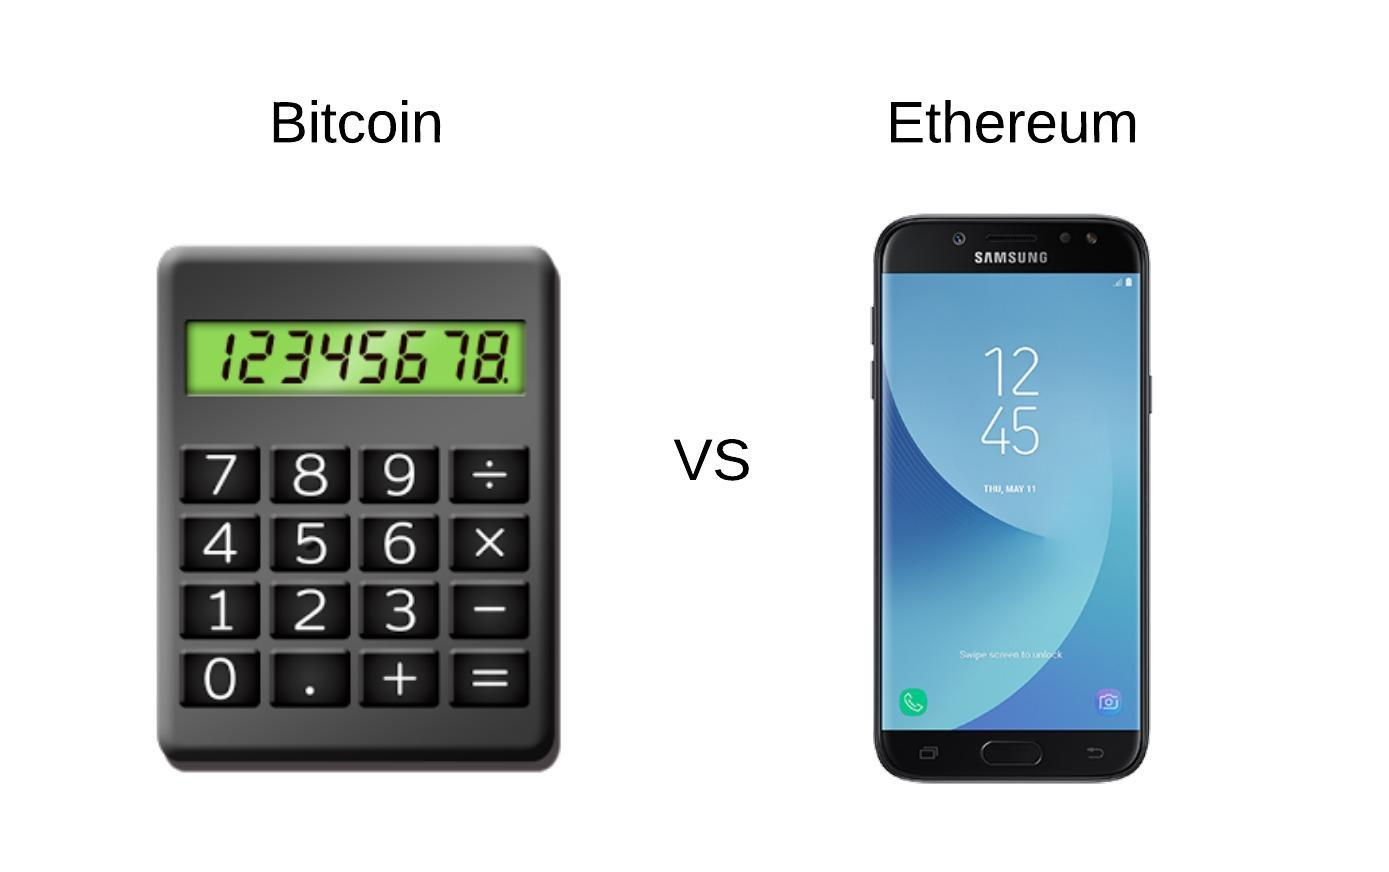
\includegraphics[scale=0.8]{gfx/bitcoinVSEthereum.jpeg}
  \caption{Bitcoin vs Ethereum}
  \label{fig:BitcoinEthereum}
\end{figure}

Furthermore, Ethereum introduces a new concept called accounts, which are unique 20-byte addresses in the blockchain. Each of these accounts has an account balance controlled by ethers (ETHs), the digital currency used by Ethereum. In Ethereum, there are two types of accounts (Figure \ref{fig:EthereumAccounts}): \newline
\textbf{(i) Externally Owned Accounts (EOAs):} These accounts normally identify a user, being controlled by their own public and private keys. Only EOA can send transactions to other accounts. A transaction in Ethereum can either send Ethers or call/trigger a contract account. \newline
\textbf{(ii) Contract accounts:} These are the accounts, where the code (smart contract) is stored. Thus, once triggered (function call from another contract), its defined code is executed.

\begin{figure}
  \centering
  	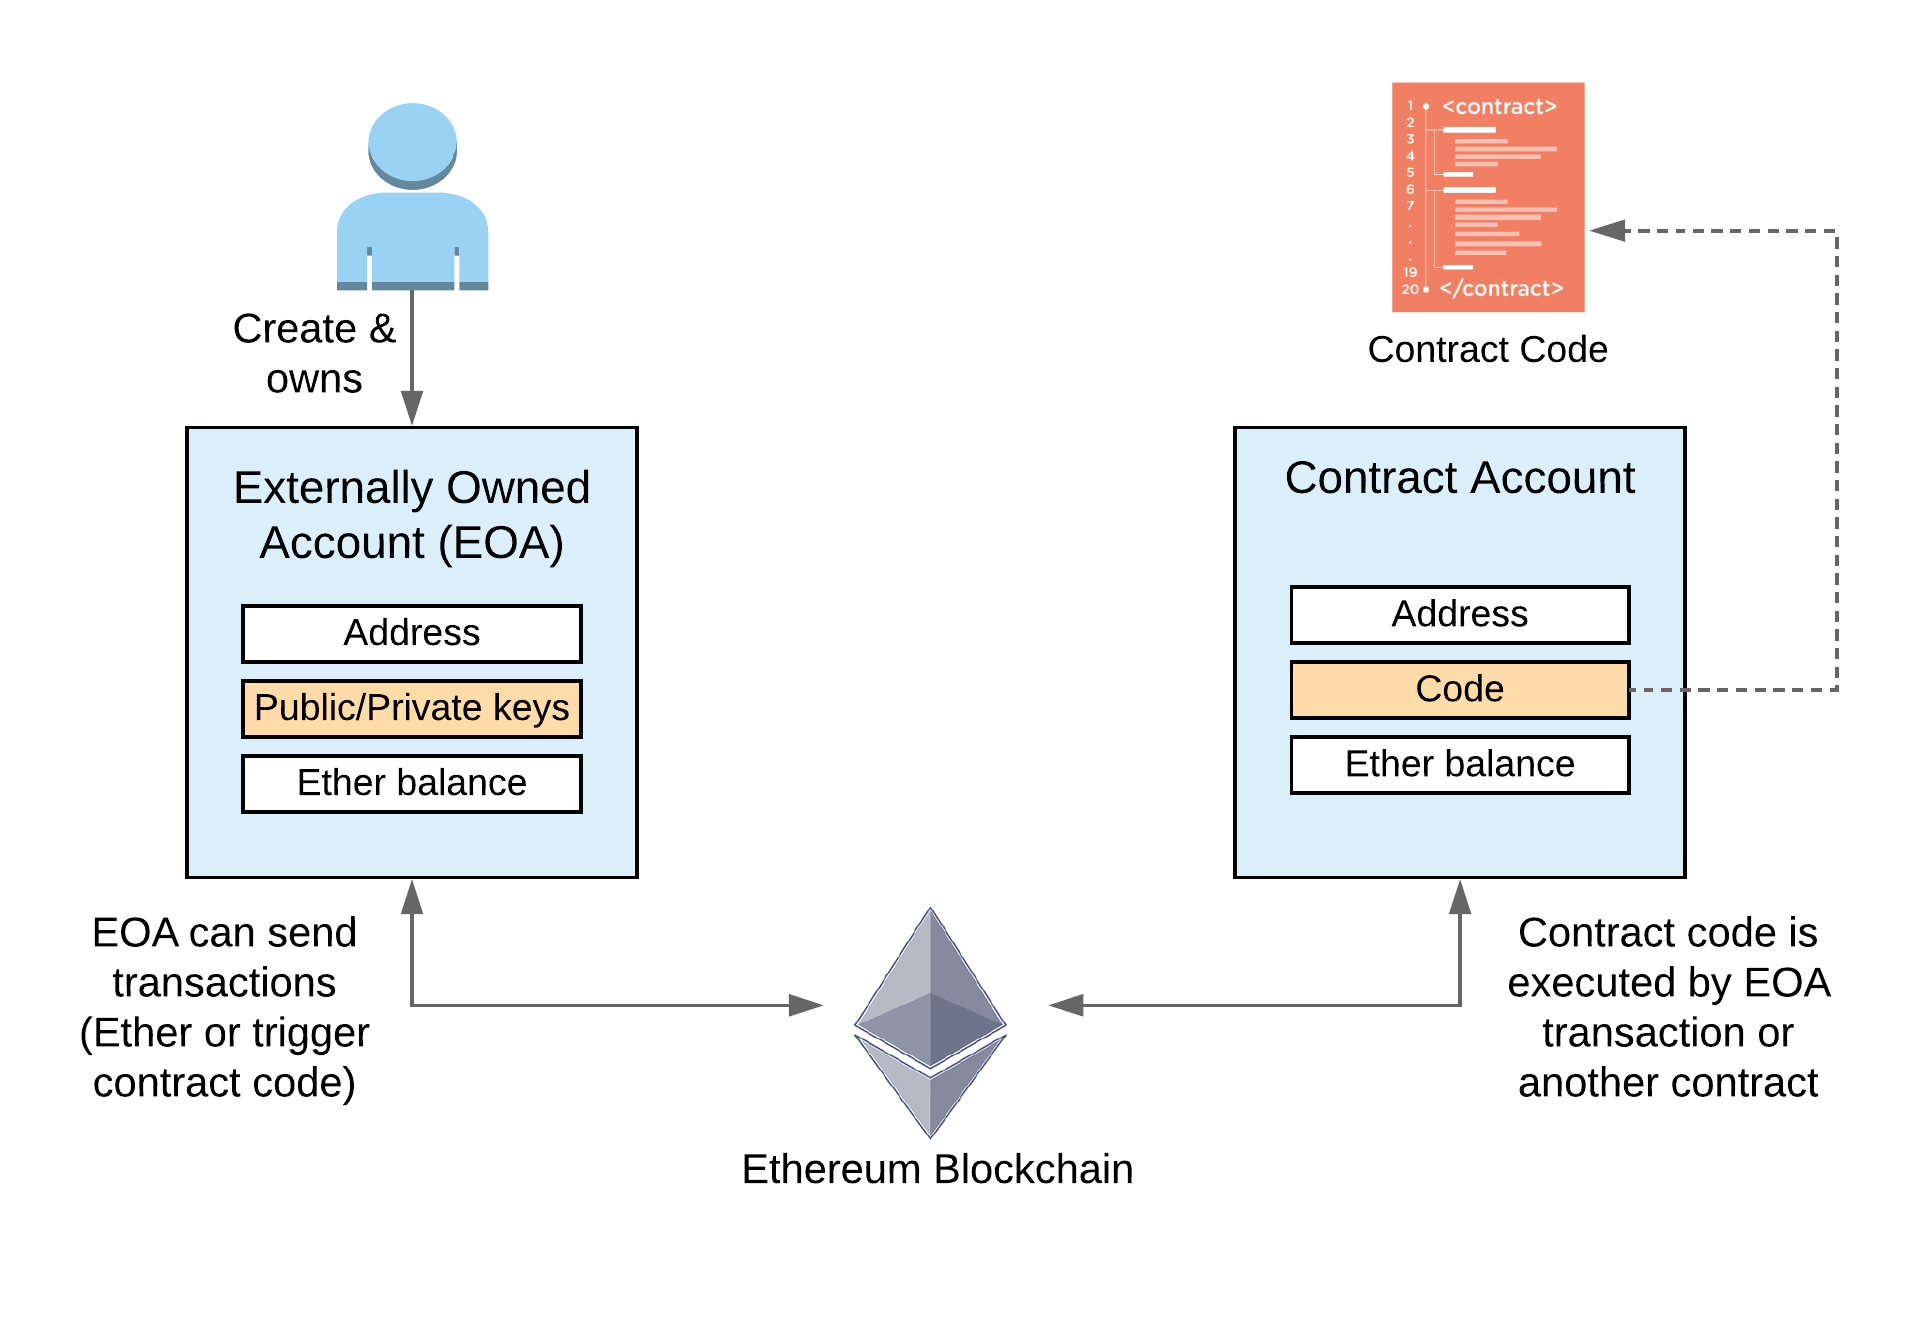
\includegraphics[scale=0.7]{gfx/ethereumAccounts.png}
  \caption{Ethereum accounts: EOA and contract accounts}
  \label{fig:EthereumAccounts}
\end{figure}

However, what happens if a code results in an infinite loop? The node will get stuck the whole time executing this contract. Solution: Ethereum uses the term "gas". Gas is an amount of ether used for executing contracts in the Ethereum blockchain. For example, if an EOA calls a contract account, which is programmed to make a money transfer to another EOA, apart from the ether transferred, it will also spend an additional amount of ether (gas). Thus, the ether used for a transaction, or transaction fee is:

$$Ether = gas price \times gas limit + value$$

Firstly, the gas limit is the maximum amount of gas that a sender is willing to spend on a transaction. Fortunately, all unused gas during a transaction (gas limit - real gas used), is refunded to the sender. Nevertheless, if a transaction gives an error, e.g: a fake transaction, this provided ether (gas limit) will never be refunded. Secondly, the gas price is its relation with real Ether, e.g: 40 Gwei (4e-8 ether). Thirdly, the value is the amount of ether transferred to the other EOA.

In conclusion, a smart contact is just an account containing code, which lives on the blockchain and allows developers to create their own decentralized applications. 

\subsubsection{Decentralized applications}

In the Ethereum white paper \cite{buterin2014next} dapps are split into three types. The first group includes financial applications, where users exchange ether in an efficient and distributed manner. The second group is formed by semi-financial applications, in which money is involved but it is mixed with data from the real world, for example with weather feed. And finally, in the third category, there are non-financial applications. For instance, an online voting platform providing a better transparency into elections, without compromising voter confidentiality.

In this paper, the blockchain technology, in particular, the Ethereum platform, will be used to approach a real-world scenario. A decentralized application (third category) that enhances supply chain performance, will be implemented. More precisely, network virtualization providers and customers will improve its communication, through the use of a web application (front-end) connected to the blockchain (back-end).


\section{Network Virtualization}

Network virtualization enables simulating hardware networks, in software. These software networks are called virtual networks, which provide flexibility, high manageability, and a low cost. Network virtualization handles two main concepts: node virtualization and link virtualization. The former implies sharing the node's physical resources located in the substrate network (e.g: CPU, storage, memory) to multiple virtual nodes from the virtual networks. The latter enables the transport of multiple virtual links in a single and shared physical link. The mentioned layers and elements involved in network virtualization, are shown in Figure \ref{fig:networkvir}, taken from \cite{carapinha2009network}.


\begin{figure}
  \centering
  	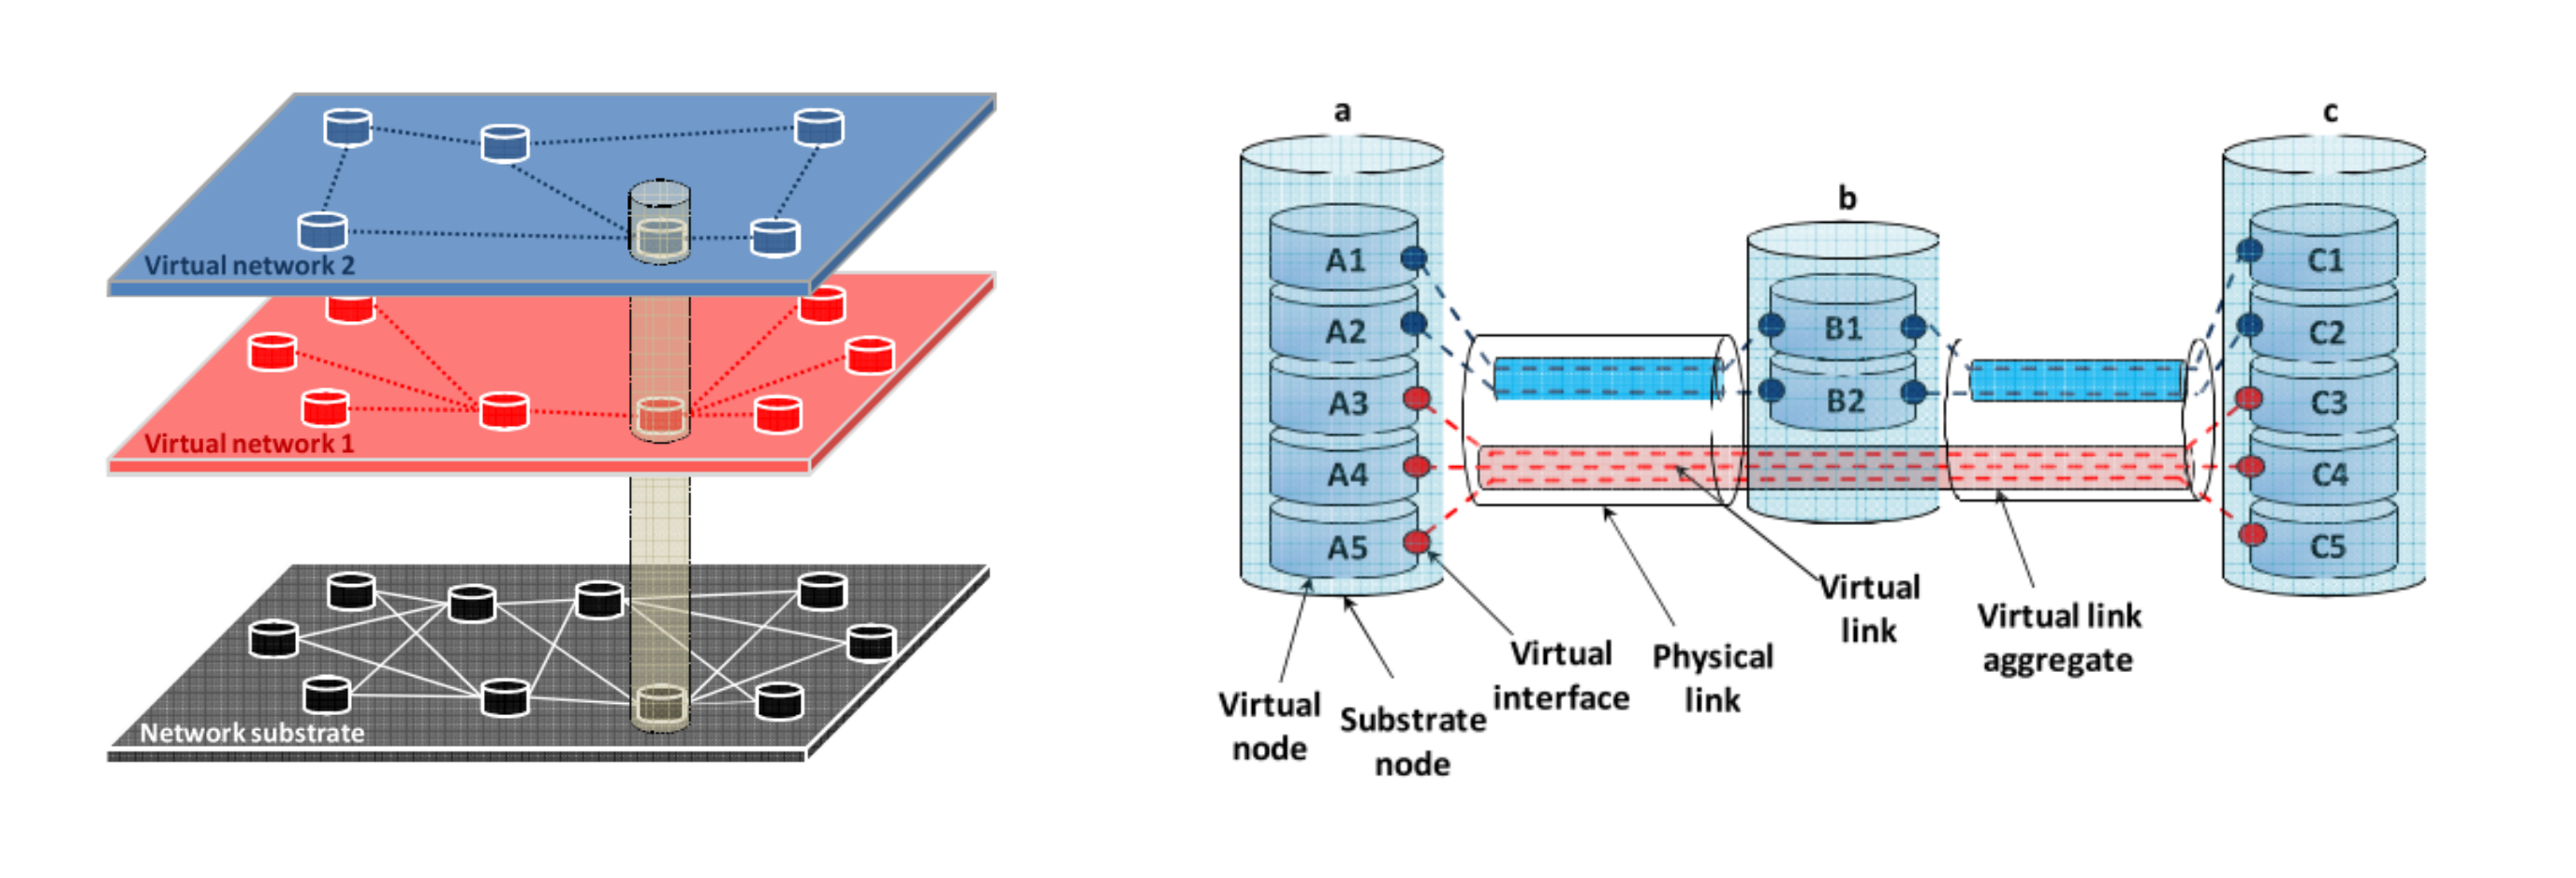
\includegraphics[scale=0.8]{gfx/networkvir.png}
  \caption{Network virtualization model and its basic elements}
  \label{fig:networkvir}
\end{figure}

In a real scenario, there are three actors participating in the network virtualization process (Figure \ref{fig:multiprov} part A): \newline
\textbf{ (i) Infrastructure providers (InPs):} Infrastructure providers (e.g: Deutsche Telekom, Telefonica) deploy and manage the physical nodes, sharing its resources to the virtual network. \newline
\textbf{ (ii) Virtual network providers: (VNPs)} Are the brokers, the intermediaries between the InPs and the service providers. \newline
\textbf{ (iii) Service Providers: (SPs)} Service providers lease virtual resources from infrastructure providers to create its own virtual network. 

In this paper a specific example of network virtualization will be investigated, where SPs are willing to embed resources among one or multiple infrastructure providers.


\subsection{Multi-Provider Virtual Network Embedding}

Multi-provider virtual network embedding consists of the allocation of virtual resources, in a constrained and limited scenario. As reported in \cite{dietrich2015multi}, the architecture suffers mainly from the limited information disclosure problem (LID), in which VNPs have a very limited knowledge of InPs internal architecture. The reason for such a problem is that the InPs are not willing to broadcast their resources information (e.g: nodes availability, cost) and network topology to the outside world. And if that was not enough, this information is crucial for the partitioning of resources in order to obtain a fair negotiation between the SPs and InPs. 

In \cite{dietrich2015multi} the LID problem is approached regarding: (i) the \textit{virtual resources availability} and (ii) the \textit{network topology}. On the one hand, virtual resources examples are obtained from Amazon EC2 \cite{amazonEC2}, which announces the attributes of different instances types (CPU, memory, cost) to give the user facility in choosing the virtual resource that better fits in its application. On the other hand, most of network topology information is treated confidentially for the InPs. Nevertheless, there are certain aspects of the network which are not considered private, such as InPs peerings (including location) and its related link cost. Thus, in the mentioned research, InPs disclose the above information using a implemented VN embedding framework that relies on an intermediary, the VN providers.

Moreover, in such scenario exists two types of communication: \newline
\textbf{Horizontal communication} is the one established between infrastructure providers to guarantee the most efficient end-services. These relations stated in \citep{zaheer2010multi}, can be: \textit{public relations} established using a market mechanism (e.g: an auction), or \textit{private relations} already arranged. In both cases, the relation arises from the need to negotiate and cooperate to serve the SPs. \newline
\textbf{Vertical communication} emerges from the negotiation between SPs and InPs, the former willing to lease some virtual resources from the latter. This communication is facilitated by a third party (VNP), an intermediary that forwards SPs request to the relevant InPs.

However, what if the SPs and InPs are not willing to trust a broker? What if they do not want to disclose any kind of information? The answer is simple: \textit{blockchain as a software connector} (Figure \ref{fig:multiprov} part B). Thanks to the blockchain, more precisely to Ethereum and smart contracts, the virtual network provider could be removed, allocating a secure and coordinated end-system. Hence, InPs disclosed information will be securely saved (public/private key cryptography) in the blockchain and just accessable for its desired users. In addition, in order to fulfill the public negotiation of virtual resources, an auction model system using smart contracts will be implemented.

\begin{figure}
  \centering
  	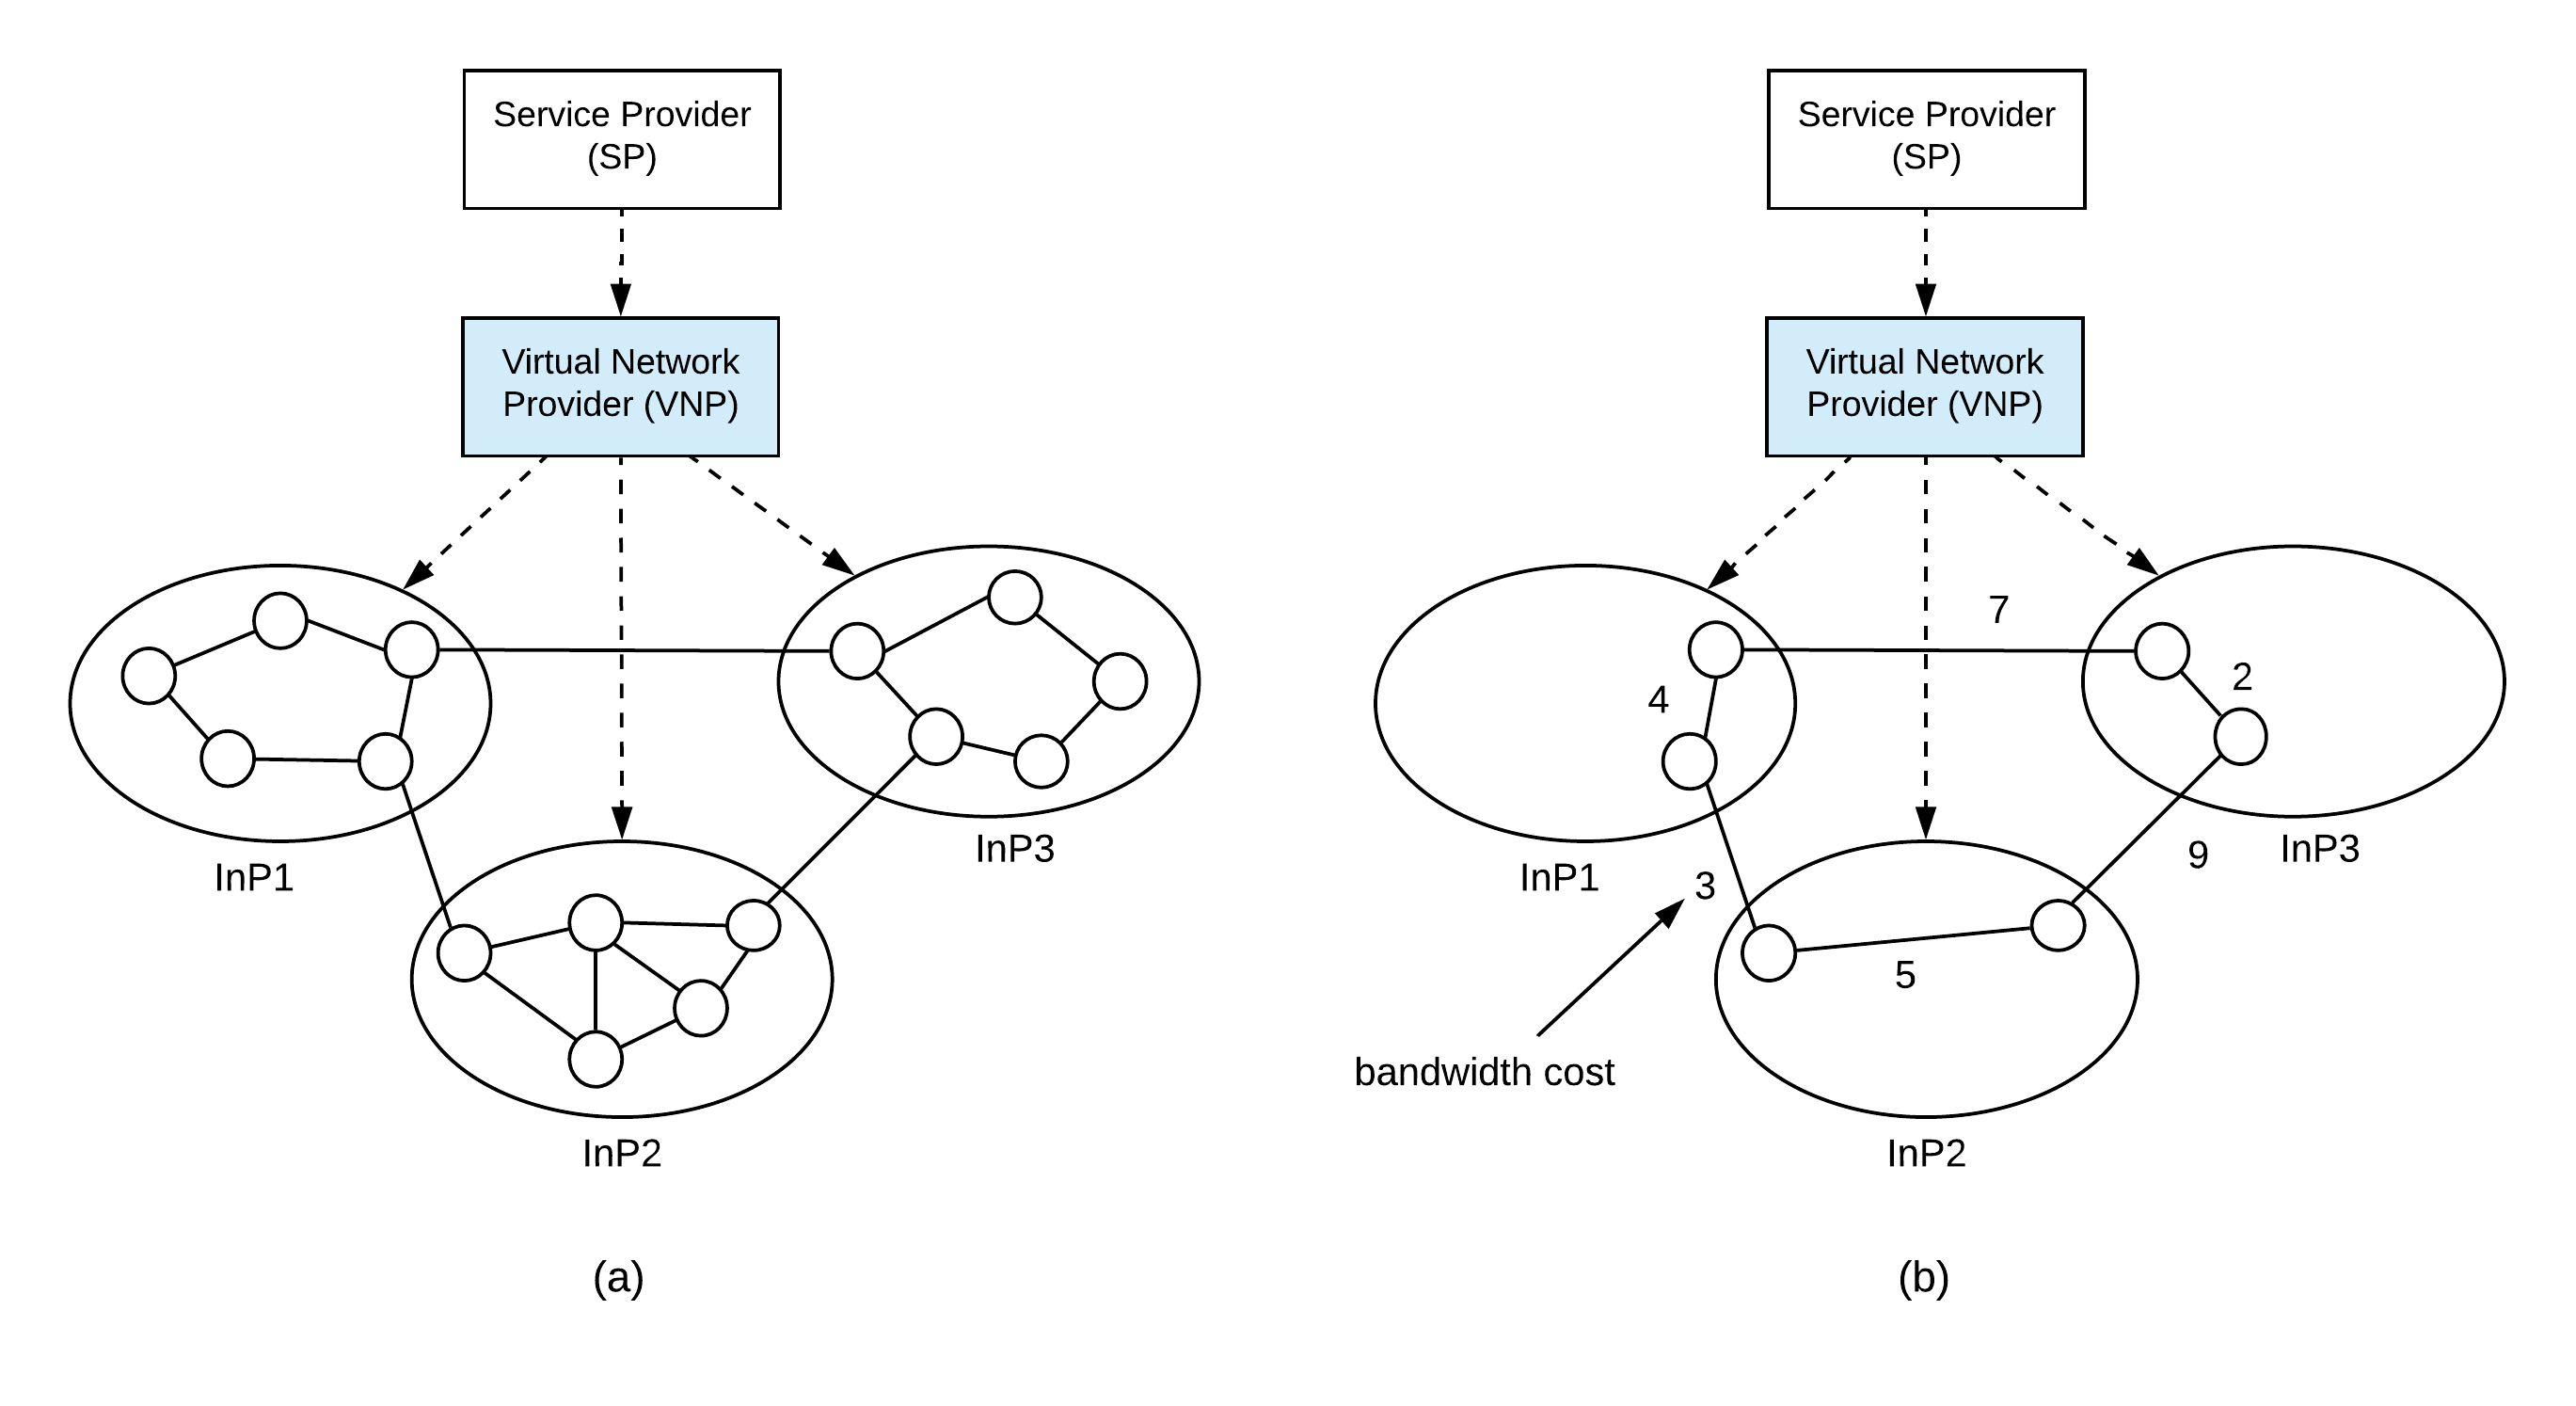
\includegraphics[scale=0.7]{gfx/multiprov.png}
  \caption{Virtual network request accross multiple InPs with and without VNP}
  \label{fig:multiprov}
\end{figure}

\section{Auction Mechanisms}

An auction is a public negotiation method involving buyers and sellers that supports market trading between P2P users. Service negotation has already been investigated in \citep{hausheer2005peermart}, \cite{ogston2002peer}, who have worked with diverse auctions platforms. While buyer's goal is to find the desired service at a low price, providers or seller's goal is to catch the attention of buyers able to pay the highest price for its offered service. Thus, an auction must provide fairness in terms of technical and economical efficiency, for both the buyer and the seller.

Firstly, auctions can be divided into: (i) \textit{one-sided auctions} where only the buyers submit their bids (e.g: a painting auctioned in an art auction), or (ii) \textit{two-sided auctions} in which buyers and sellers submit their bids. Normally, when any of the two sides (buyer or seller) cannot performe a good estimatation of the service, a one-side auction is preferred. Secondly, the auctions are: (i) (i) \textit{open-bid} auctions, as it name suggests, the bids are publicly open to the other bidders or (ii) \textit{sealed-bid} auctions where the bids are kept secret in the system.

Accordingly, a \textit{sealed one-side auction} is the one which best meets our system specifications, since the InPs do not want to disclose their network topology or nodes information. Our auction procedure will start with the SP requesting a virtual network (a graph of virtual nodes) along with an upper bound, the last being the maximum amount of money the SP is willing to pay. Then, the InPs will estimate the request requirements (e.g: nodes availability or costs) in their infrastructure and thereafter submit their bids. In other words, the InPs will be sellers submitting bids and SPs the consumers requesting a service. Despite it can be seen as a fair system, how can the SP ensure that the InPs are offering prices proportional to the current market costs?

\subsection{Vickrey Auction Model}

Many types of auction models exist, such as the English or Dutch auctions \cite{coppinger1980incentives}, however as previously discussed a fair-price system is extremely needed. The Vickrey auction model matches these requirements, achieving a reasonable price for the buyer by motivating bidders to bid truthfully. One of the Vickrey auction model important aspects is that corresponds to a \textit{second-price} auction. In a second-price auction the bidder (InP) will offer a price for the service, and among all the bids, the lowest one will win the auction. Nevertheless, the service will be rendered at the second lowest bid. It is important to note that in our scenario the lowest auction wins and not the highest. The reason is that at the end the SPs is who will pay the bid value. For instance, suppose that all the InPs make an offer close to the upper bound specified by the SP. If the highest bid wins, the SPs will always end-up paying approximately its upper bound (unfair). However, if the lowest bid wins, the system ensures that the InPs submits a bid proportional to the real cost since it will be the minimum amount of money that they could earn.

In addition, as previously introduced, the Vickrey auction has the particularity of being a second-price one. From the bidder point of view means that he can safely bid the true value, knowing that if he wins, he will earn more than his bid. Thus, no InP bidder ends up earning less than what they have committed. However, the second-price concept needs to be thoroughly investigated as long as a bidder can submit multiple bids. Imagine an scenario, where a single bidder A submits two bids: \{1 \euro,9 \euro\} for a service with a real cost 5 \euro. In this case, the buyer will end up paying 9 for the service. Therefore, the second-price auction model needs always to be compared between bidders and not between bids. Suppose the last example, with a second bidder B submitting \{5 \euro, 6 \euro\}. At the end user A, will win the bid but earning 5 \euro, risking that if he would have been the only user bidding, he will earn no more than 1 \euro.

Ultimately, after examining the different attacker scenarios along with the pros and cons of each auction type and model, the \textbf{\textit{two-sided and sealed Vickrey auction}} fulfills the application requirements.  


\section{Summary}


%*****************************************
\chapter{Related Work}
\label{ch:relatedwork}
%*****************************************
\hint{This chapter should give a comprehensive overview on the related work done by other authors followed by an analysis why the existing related work is not capable of solving the problem described in the introduction.
The chapter should have a length of about three to five pages!}
\section{Related Work Area 1}

IOTA-TANGLE VS BLOCKCHAIN VS DATABASE

\section{Related Work Area 2}

OTHER PAPERS IN Multi-provider network embedding
\section{Analysis of Related Work}

\section{Summary}

%*****************************************
\chapter{Design}
\label{ch:design}
%*****************************************
\hint{This chapter should describe the design of the own approach on a conceptional level without mentioning the implementation details. The section should have a length of about five pages.}

GETH vs ETH NW, web3, Solidity, truffle ...

\section{Requirements and Assumptions}

\section{System Overview}


\subsection{Blockchain types}


\subsection{Component 1}

\subsection{Component 2}

\section{Summary}

%*****************************************
\chapter{Implementation}

How a contract is compiled in to the Ethereum BC.
\label{ch:implementation}
%*****************************************

\hint{This chapter should describe the details of the implementation addressing the following questions: \\ \\
1. What are the design decisions made? \\
2. What is the environment the approach is developed in? \\
3. How are components mapped to classes of the source code? \\
4. How do the components interact with each other?  \\
5. What are limitations of the implementation? \\ \\
The section should have a length of about five pages.}
\section{Design Decisions}

\section{Architecture}

\section{Interaction of Components}

\section{Summary}

%*****************************************
\chapter{Evaluation}
\label{ch:evaluation}
%*****************************************
\hint{This chapter should describe how the evaluation of the implemented mechanism was done. \\ \\
1. Which evaluation method is used and why? Simulations, prototype? \\
2. What is the goal of the evaluation? Comparison? Proof of concept? \\
3. Wich metrics are used for characterizing the performance, costs, fairness, and efficiency of the system?\\
4. What are the parameter settings used in the evaluation and why? If possible always justify why a certain threshold has been chose for a particular parameter.  \\
5. What is the outcome of the evaluation? \\ \\
The section should have a length of about five to ten pages.}
\section{Goal and Methodology}

\section{Evaluation Setup}

\section{Evaluation Results}

\section{Analysis of Results}


%*****************************************
\chapter{Conclusions}
\label{ch:closure}
%*****************************************

\hint{This chapter should summarize the thesis and describe the main contributions of the thesis. Subsequently, it should describe possible future work in the context of the thesis. What are limitations of the developed solutions? Which things can be improved?
The section should have a length of about three pages.}

\section{Summary}

\section{Contributions}

\section{Future Work}

\section{Final Remarks}
